\chapter{The Visual Atlas of Inscribed Polygons}
\label{chap:visual-atlas}

\section*{Cartographic Conventions}

This catalogue displays the complete census of non-equivalent
dihedral inscribed polygons across the circular rings $\mathbb{Z}_1$
through $\mathbb{Z}_{16}$, organized sequentially ring by ring.

Each drawing portrays an individual dihedral orbit in its canonical orientation:
\begin{itemize}
    \item \textbf{Lattice Geometry}: The ambient circular lattice $\mathbb{Z}_n$ is the regular $n$-gon with vertex $0$ positioned at the top and indices advancing clockwise $0, 1, \dots, n-1$. Faint pips mark unselected vertices.
    \item \textbf{Polygonal Hierarchy}:
    \begin{itemize}
        \item \emph{Empty Polygons ($k=0$)} are marked by an ambient wireframe with a central null indicator.
        \item \emph{Unigons ($k=1$)} are marked by a prominent circular node at the active vertex.
        \item \emph{Digons ($k=2$)} are drawn as bold lines connecting the vertex pair.
        \item \emph{Polygons ($k \ge 3$)} are drawn as shaded polygonal tiles bounded by perimeter chords and solid vertex nodes.
    \end{itemize}
    \item \textbf{Bilateral Symmetry Colouring}:
    \begin{itemize}
        \item \textbf{Blue}: Bilaterally symmetric (achiral) polygons have (at least) one internal axis of dihedral reflection.
        \item \textbf{Pink}: Scalene (chiral) polygons lack reflection symmetry.
    \end{itemize}
    \item \textbf{Coordinate Annotations}:
    \begin{itemize}
        \item \textbf{Upper-Left Designation}: Bold cardinality-and-rank index ($k\text{-}i$) indicates the $i$-th non-equivalent $k$-gon on the active lattice ring, cross-referenced with the analytical dataset.
        \item \textbf{Lower-Right Orbit Size}: Dihedral orbit length $|\mathcal{O}| \in \{1, 2, \dots, 2n\}$ under the action of $D_n$.
    \end{itemize}
\end{itemize}

\bigskip
\noindent\textit{Degenerate Base Lattices}: The unigonal and digonal configurations on the degenerate rings $\mathbb{Z}_1$ and $\mathbb{Z}_2$ are illustrated in Figure~\ref{fig:degenerate-rings} of Chapter~\ref{chap:polygon-geometry}. The visual atlas plates begin with the triangular ring $\mathbb{Z}_3$ on Plate~1.

\clearpage
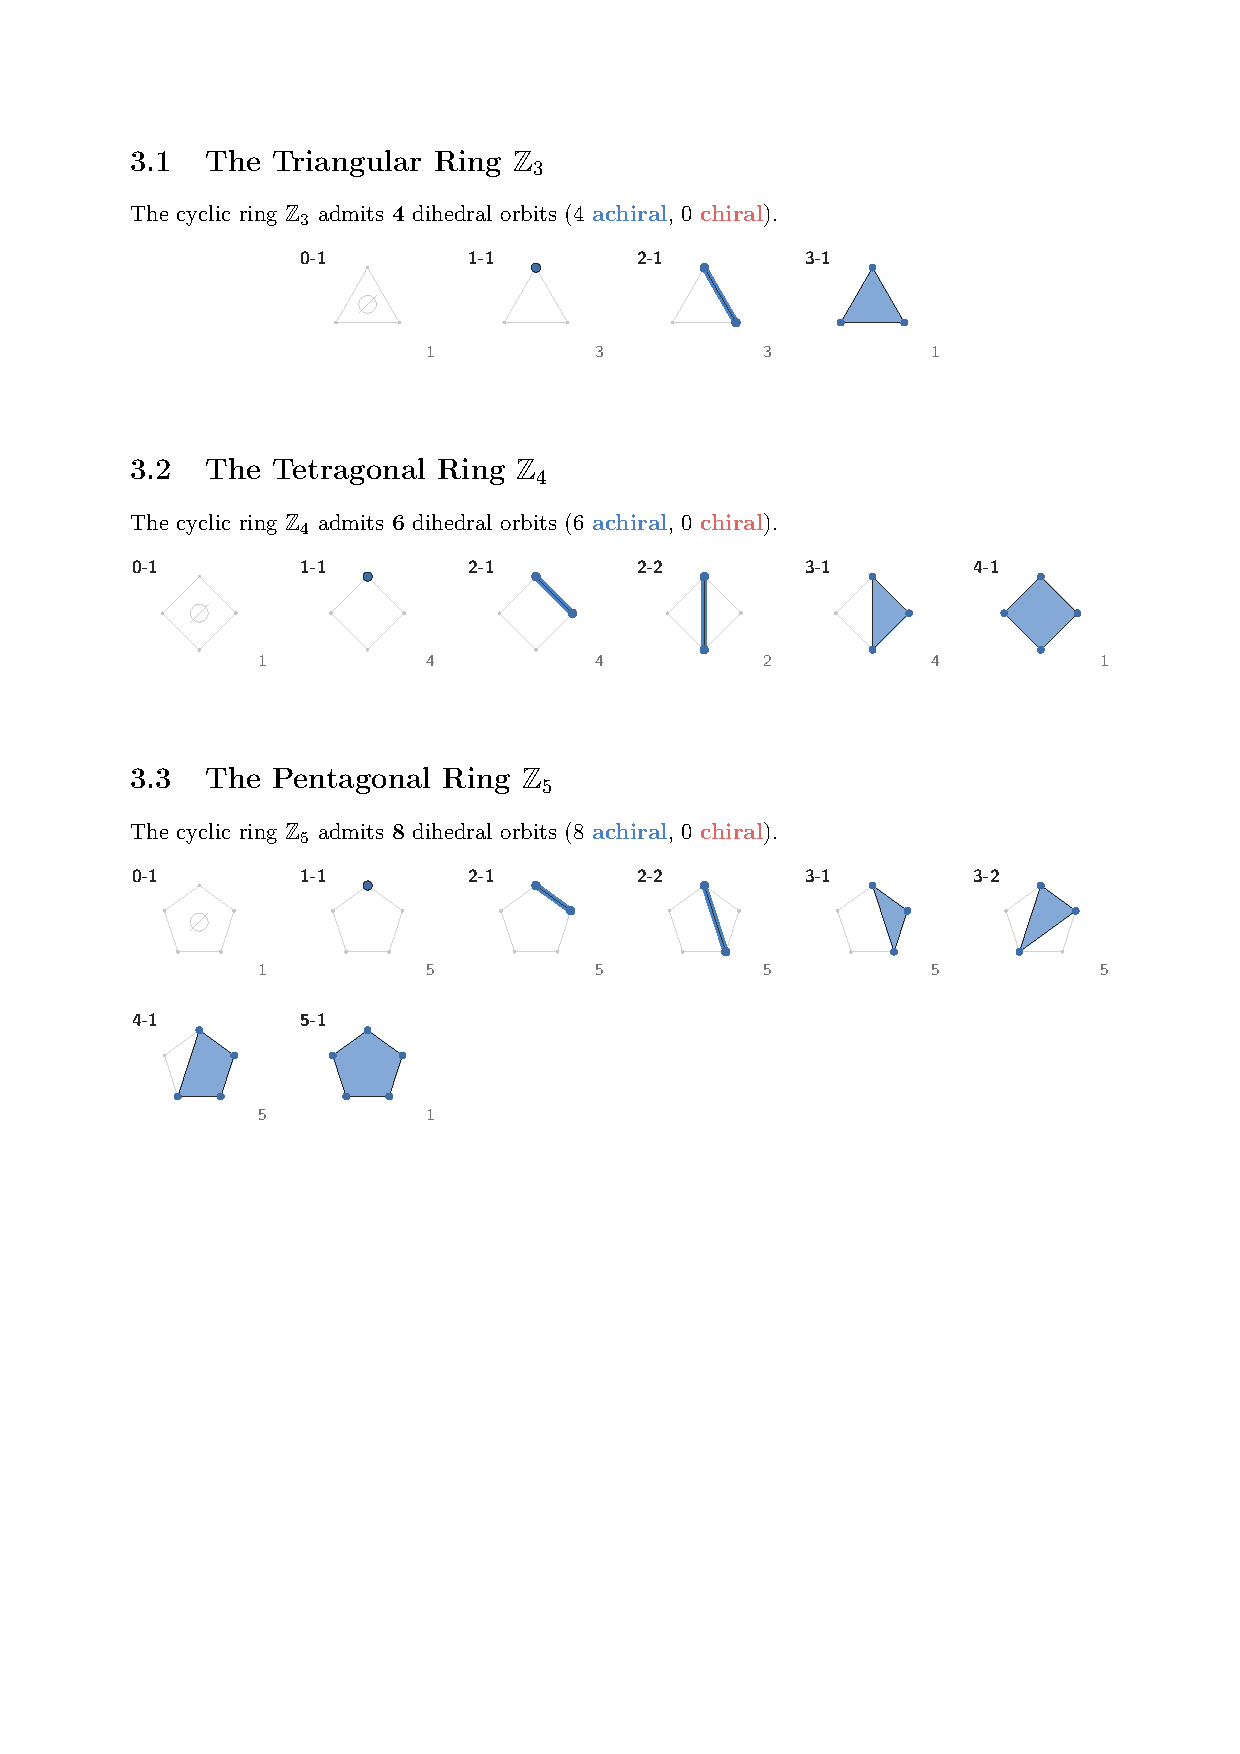
\includepdf[
  pages=-,
  pagecommand={\thispagestyle{headings}},
  addtotoc={
     1, section, 1, {The Triangular Ring \texorpdfstring{$\mathbb{Z}_3$}{Z3}}, sec:ring-z3,
     1, section, 1, {The Tetragonal Ring \texorpdfstring{$\mathbb{Z}_4$}{Z4}}, sec:ring-z4,
     1, section, 1, {The Pentagonal Ring \texorpdfstring{$\mathbb{Z}_5$}{Z5}}, sec:ring-z5,
     2, section, 1, {The Hexagonal Ring \texorpdfstring{$\mathbb{Z}_6$}{Z6}}, sec:ring-z6,
     2, section, 1, {The Heptagonal Ring \texorpdfstring{$\mathbb{Z}_7$}{Z7}}, sec:ring-z7,
     3, section, 1, {The Octagonal Ring \texorpdfstring{$\mathbb{Z}_8$}{Z8}}, sec:ring-z8,
     4, section, 1, {The Enneagonal Ring \texorpdfstring{$\mathbb{Z}_9$}{Z9}}, sec:ring-z9,
     5, section, 1, {The Decagonal Ring \texorpdfstring{$\mathbb{Z}_{10}$}{Z10}}, sec:ring-z10,
     7, section, 1, {The Hendecagonal Ring \texorpdfstring{$\mathbb{Z}_{11}$}{Z11}}, sec:ring-z11,
    10, section, 1, {The Dodecagonal Ring \texorpdfstring{$\mathbb{Z}_{12}$}{Z12}}, sec:ring-z12,
    15, section, 1, {The Tridecagonal Ring \texorpdfstring{$\mathbb{Z}_{13}$}{Z13}}, sec:ring-z13,
    23, section, 1, {The Tetradecagonal Ring \texorpdfstring{$\mathbb{Z}_{14}$}{Z14}}, sec:ring-z14,
    36, section, 1, {The Pentadecagonal Ring \texorpdfstring{$\mathbb{Z}_{15}$}{Z15}}, sec:ring-z15,
    59, section, 1, {The Hexadecagonal Ring \texorpdfstring{$\mathbb{Z}_{16}$}{Z16}}, sec:ring-z16
  }
]{plates/poly_plates.pdf}
